\begin{figure}[h!]
	\begin{tikzpicture}
		% Diagram setup
		\tkzKiviatDiagram[scale=1.0,label distance=.5cm,
			radial  = 4,
			gap     = 1,  
			lattice = 4]{
				Plattformabhängigkeit,
				Installation,
				Speicherzugriff,
				Speicherbedarf,
				Aktualisierbarkeit,
				Design,
				Bibliotheken,
				Umsetzung,
				Testbarkeit,
				Vorausgesetzte Entwicklungserfahrung			
			}
		
		% native App
		\tkzKiviatLine[thick,color=blue,mark=ball,
		fill=blue!20,opacity=.5](1,4,4,3,3,3,3,4,2,3)
		
		% PWA
		\tkzKiviatLine[thick,color=green,mark=ball,
		fill=green!20,opacity=.5](3,2,3,4,4,1,4,4,4,1)		

		% Legende -- - + ++
		\foreach \X [count=\Y]in {$--$, $-$, \Circle, $+$, $++$}
		\node[anchor=north,rotate=0] at (\Y-1,0) {\X};

	\end{tikzpicture}
	
	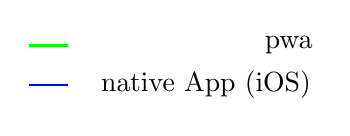
\begin{tikzpicture}	
		% Legende PWA
		\draw [thick, green] (0,0.5) -- (0.5,0.5); 
		\node at (3.3,0.5) {\acf{pwa}};
		
		% Legende iOS
		\draw [thick, blue] (0,0) -- (0.5,0); 
		\node at (2.25,0) {native App (iOS)};	
	\end{tikzpicture}
	
	\caption{Kriterienvergleich im Netzdiagram (\acs{pwa} und native App)}
\end{figure}